\section*{Scenario C: Reduced mobility}
In this simulation we are interested in the result what happens if we reduce the movement parameter to $\sigma = 0.05$.
When looking at Figure~\ref{fig:ex03}, the rabbits population exhibits multiple very high peaks, reaching even higher numbers than in exercise A, even though we have the same reproduction and mortality parameters.
The following key observation can be made about the system
\begin{itemize}
	\item The rabbit population has extreme booms and crashes (compared to exercise A) with peaks being roughly 10 times higher.
	\item As seen before the wolf population shows a delayed response, with way smaller peaks.
	\item The small movement parameter limits the mixing of population.
\end{itemize}
Looking at the species in more detail we can draw the following conclusions:
\begin{itemize}
	\item Wolves are unable to effectively find rabbits across the domain, resulting in areas where the rabbit population can grow unchecked.
	\item Rabbits are able to form dense reproductive clusters, resulting in extremely high booms of rabbit population.
	\item The eventual crash is likely caused by a wolf being eventually able to reach the hotspot of rabbits, leading to a rapid crash of rabbits due to the abundance of rabbits for the wolf to eat and therefore being able to reproduce.
\end{itemize}
The classic Lotka-Volterra model is in this scenario a rather poor approximation of the system dynamics, as the assumption of well-mixed populations is severely violated. The extreme spikes in population demonstrate how spatial effects can dominate the systems behaviour when movement is constrained. We create a boom-bust cycles which is driven by the positions of the predators and prey instead of an interaction driven feedback mechanism captured in the differential equations \eqref{eq:lv}.
\begin{figure}[H]
	\centering
	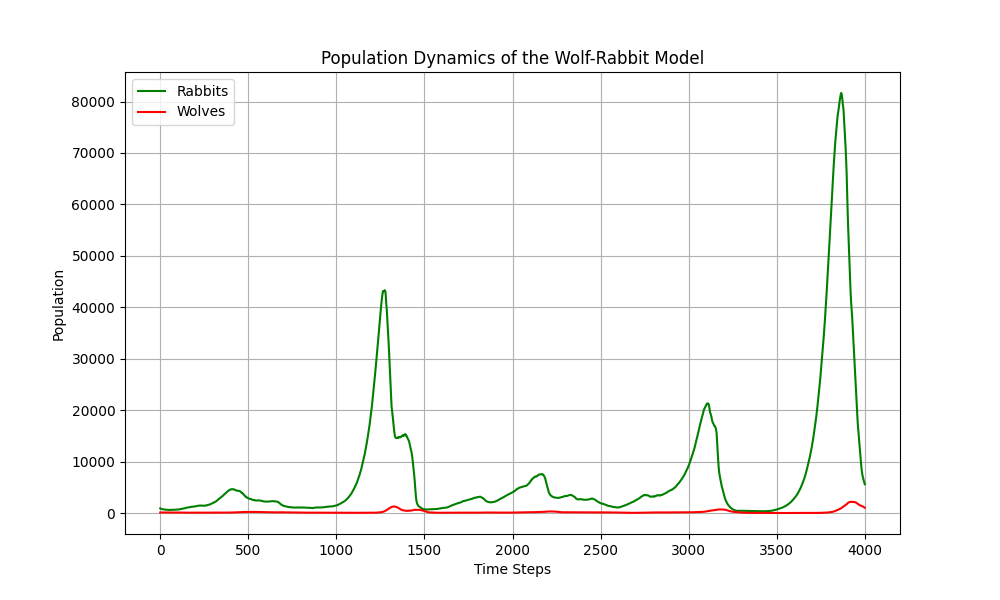
\includegraphics[width=\textwidth]{./media/population_dynamics_ex03.png}
	\caption{
		\textbf{Population Dynamics}
		$L = 8$, $\sigma = 0.05$
	}
	\label{fig:ex03}
\end{figure}
\section*{Conclusion}
This agent-based simulation of the predator-prey dynamics showed several significant insights that extend beyond the classical the Lotka-Volterra models. The incorporation of spatial heterogeneity, stochastic movement, and interactions on an individual level, we observed wide variety of behaviors across different configurations.
\newline
\newline
In Scenario A, we observed the expected patterns with a phase difference between predator and prey populations. However, the spatial component of our model caused a  more complex dynamics compared to what the  differential equations would predict. This included non-uniform oscillations and extreme population counts after the 2500-time step mark. \newline
By reducing the rabbit lifespan in Scenario B, we were able to observe the critical importance of prey longevity to ecosystem stability. Rather than oscillations, the system experienced a complete collapse. This highlights the importance of threshold effects and critical population densities.\newline
Perhaps most interesting result were obtained in Scenario C, where we observed extreme peaks and crashes of rabbit populations, by reducing the mobility. By creating "safe zones", where prey can multiply unchecked until eventually intruded by predators, leading to boom-bust cycles on an order of magnitude more extreme than in Scenario A.
\newline
\newline
The most important findings can be boiled down to the following points:

\begin{itemize}
	\item Spatial dynamics and the movement of individual agents highly influence population stability, probably even more than reproduction or mortality rates.
	\item There is a high parameter sensitivity in predator-prey, small changes can cause regime shifts from stable oscillations to extinction or extreme fluctuations.
	\item The addition of spatial heterogeneity reveals dynamics that which are not present in traditional Lotka-Volterra models, clearly points out  the importance of agent-based approaches.
\end{itemize}
For future work this rather simple simulation could be extend by incorporating multiple ecological complexities. This could include food for rabbits that grows and depletes, terrain heterogeneity, introducing sexes for mating, adapting behaviour of agents among others. These extensions would further bridge the gap between theoretical models and the complex dynamics observed in the real world.
